\documentclass[12pt,compress,aspectratio=169]{beamer}

\usetheme{metropolis}
\setbeamersize{text margin left=.5cm,text margin right=.5cm}

\usefonttheme{professionalfonts}
\usepackage{amsmath}
\usepackage{siunitx}
\usepackage{tikz}
\usepackage{mathpazo}

\usetikzlibrary{patterns}

\setsansfont{Roboto Light}
\setmonofont{Ubuntu Mono}
\setlength{\parskip}{0pt}
\setlength{\itemsep}{0pt}
\renewcommand{\baselinestretch}{1}

\sisetup{
  detect-all,
  math-sf=\textsf,
  number-math-rm=\mathnormal,
  per-mode=symbol
}

\title{Topic 5: Circular Motion}
\subtitle{Advanced Placement Physics 1}
\author[TML]{Dr.\ Timothy Leung}
\institute{Olympiads School}
\date{\today}

\newcommand{\pic}[2]{\includegraphics[width=#1\textwidth]{#2}}
\newcommand{\mb}[1]{\ensuremath\mathbf{#1}}
\newcommand{\eq}[2]{\vspace{#1}{\Large\begin{displaymath}#2\end{displaymath}}}


\begin{document}

\begin{frame}
  \maketitle
\end{frame}


\begin{frame}{Files to Download}
  Please download the following files from the school website if you have not
  already done so:
  \begin{itemize}
  \item\texttt{PhysAP1-05-circMotion.pdf}---The ``print version'' of the
    class slides for this topic.
  \item\texttt{PhysAP1-05-Homework.pdf}---Homework problems for this topic.
  \end{itemize}
  \vspace{.1in}Please download/print the PDF file for the class slides before
  each class. There is no point copying notes that are already on the slides.
  Instead, focus on things that aren't necessarily on the slides. If you wish
  to print the slides, we recommend printing 4 slides per page.
\end{frame}



\begin{frame}{Review of Circular Motion}
  In \textbf{circular motion}, an object of mass $m$ moves in a circular path
  about a fixed center. In Grade 12 Physics, you were introduced to
  \emph{uniform} circular motion, where:
  \begin{itemize}
  \item the object's speed (magnitude of velocity) is constant
  \item the object's \textbf{centripetal acceleration} is toward the center
  \item the object's acceleration is caused by a \textbf{centripetal force}
  \end{itemize}
\end{frame}



%\section{Polar Coordinates}
%
%\begin{frame}{Polar Coordinate System in 2D}
%  \begin{columns}
%    \column{.32\textwidth}
%    \begin{tikzpicture}[scale=.75]
%      \draw[->](-3,0)--(3,0) node[pos=1,right]{\footnotesize$x$};
%      \draw[->](0,-3)--(0,3) node[pos=1,above]{\footnotesize$y$};
%      \draw (0,0) circle(2.5);
%      \begin{scope}[rotate=38]
%        \draw[->] (0,0)--(2.45,0) node[midway,above]{\footnotesize$r$};
%        \draw[fill=red!60] (2.5,0) circle(.1);
%      \end{scope}
%      \draw(1.5,0)[->] arc(0:38:1.5) node[pos=.55,right]{\footnotesize$\theta$};
%    \end{tikzpicture}
%
%    \column{.68\textwidth}
%    In the Cartesian coordinate system for rectilinear motion, an object's
%    position is described by its $x$ and $y$ coordinates:
%
%    \eq{-.25in}{
%      \mb{x}(x,y)
%      }
%
%    \vspace{-.15in}For circular motion, the \textbf{polar coordinate system} is
%    preferred. The position of an object can also be described by:
%
%    \eq{-.25in}{
%      \mb{r}(r,\theta)
%    }
%
%    \vspace{-.1in}Where $r$ is distance from the origin, and $\theta$ is the
%    standard angle, measured counterclockwise from the $x$ axis in
%    \emph{radians}
%  \end{columns}
%\end{frame}
%
%
%
%\begin{frame}{Polar Coordinate System in 2D}
%  \begin{columns}
%    \column{.3\textwidth}
%    \begin{tikzpicture}[scale=.75]
%      \draw[->](-3,0)--(3,0) node[pos=1,right]{\footnotesize$x$};
%      \draw[->](0,-3)--(0,3) node[pos=1,above]{\footnotesize$y$};
%      \draw (0,0) circle(2.5);
%      \begin{scope}[rotate=38]
%        \draw[->] (0,0)--(2.45,0) node[midway,above]{\footnotesize$r$};
%        \draw[fill=red!60] (2.5,0) circle(.1);
%      \end{scope}
%      \draw(1.5,0)[->] arc(0:38:1.5) node[pos=.55,right]{\footnotesize$\theta$};
%    \end{tikzpicture}
%
%    \column{.7\textwidth}
%    \begin{itemize}
%    \item This is consistent with how position vectors are expressed in
%      Grade 11/12 Physics: magnitude ($r$) and direction ($\theta$)
%    \item Cartesian coordinates can be obtained from the polar coordinates:
%      
%      \eq{-.3in}{
%        x=r\cos\theta\quad y=r\sin\theta
%      }
%    \item While polar coordinates can be obtained from Cartesian coordinates:
%
%      \eq{-.25in}{
%        r=\sqrt{x^2+y^2}\quad\text{\normalsize and}\quad\tan\theta=\frac{y}{x}
%      }
%      
%    \end{itemize}
%  \end{columns}
%\end{frame}



\section{Rigid-Body Circular Motion}

\begin{frame}{Angular Position and Angular Velocity}
  \vspace{.2in}
  \begin{columns}
    \column{.32\textwidth}
    \begin{tikzpicture}[scale=.75]
      \draw[->](-3,0)--(3,0) node[pos=1,right]{\footnotesize$x$};
      \draw[->](0,-3)--(0,3) node[pos=1,above]{\footnotesize$y$};
      \draw (0,0) circle(2.5);
      \begin{scope}[rotate=38]
        \draw[->] (0,0)--(2.44,0) node[midway,above]{\footnotesize$r$};
        \draw[fill=red!60] (2.5,0) circle(.1);
      \end{scope}
      \draw(1,0)[->] arc(0:38:1) node[midway,right]{\footnotesize$\theta$};
    \end{tikzpicture}
    
    \column{.68\textwidth}
    For circular motion with constant radius $r$, the \textbf{angular position}
    $\theta(t)$ fully describes an object's position. It is generally measured
    in radians (rad):
      
    \eq{-.25in}{
      \boxed{\theta=\theta(t)}
    }
    
    \textbf{Average angular velocity} $\overline{\omega}$ (or
    \textbf{angular frequency}) is the change in angular position over a finite
    time interval. It is measured in \si{rad\per\second}.
    
    \eq{-.2in}{
      \boxed{\overline{\omega}=\frac{\Delta\theta}{\Delta t}}
    }

  \end{columns}
\end{frame}



\begin{frame}{Velocity and Angular Velocity}
  \begin{columns}
    \column{.35\textwidth}
    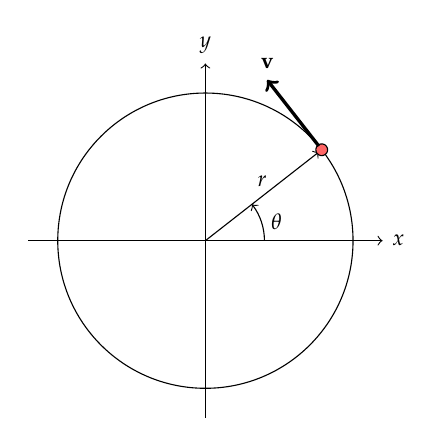
\begin{tikzpicture}[scale=.75]
      \draw[->](-3,0)--(3,0) node[pos=1,right]{\footnotesize$x$};
      \draw[->](0,-3)--(0,3) node[pos=1,above]{\footnotesize$y$};
      \draw (0,0) circle(2.5);
      \begin{scope}[rotate=38]
        \draw[->] (0,0)--(2.44,0) node[midway,above]{\footnotesize$r$};
        \draw[fill=red!60] (2.5,0) circle(.1);
        \draw[very thick,->](2.5,.08)--(2.5,1.5)
        node[pos=1,above]{\footnotesize$\mb{v}$};
      \end{scope}
      \draw(1,0)[->] arc(0:38:1) node[midway,right]{\footnotesize$\theta$};
    \end{tikzpicture}

    \column{.65\textwidth}
    The actual velocity of an object in circular motion is related to the
    angular velocity by:

    \eq{-.3in}{
      v(t)=r\omega(t)
    }    

    \begin{itemize}
    \item\vspace{-.25in} The direction of $\mb{v}$ is tangent to circle
    \item If $\omega>0$, the motion is counter-clockwise
    \item If $\omega<0$, the motion is clockwise
    \end{itemize}
  \end{columns}
\end{frame}



\begin{frame}{Period \& Frequency}
  \begin{columns}
    \column{.3\textwidth}
    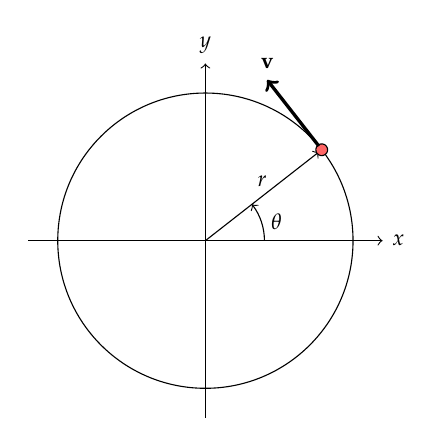
\begin{tikzpicture}[scale=.75]
      \draw[->](-3,0)--(3,0) node[pos=1,right]{\footnotesize$x$};
      \draw[->](0,-3)--(0,3) node[pos=1,above]{\footnotesize$y$};
      \draw (0,0) circle(2.5);
      \begin{scope}[rotate=38]
        \draw[->] (0,0)--(2.44,0) node[midway,above]{\footnotesize$r$};
        \draw[fill=red!60] (2.5,0) circle(.1);
        \draw[very thick,->](2.5,.08)--(2.5,1.5)
        node[pos=1,above]{\footnotesize$\mb{v}$};
      \end{scope}
      \draw(1,0)[->] arc(0:38:1) node[midway,right]{\footnotesize$\theta$};
    \end{tikzpicture}

    \column{.7\textwidth}
    For a constant $\omega$ (uniform circular motion), the motion is strictly
    periodic; its \textbf{frequency} $f$ and \textbf{period} $T$ given by:

    \eq{-.15in}{
      \boxed{f=\frac{\omega}{2\pi}}\quad
      \boxed{T=\frac{2\pi}{\omega}}\quad
      \boxed{f=\frac1T}
    }
    
    $T$ is measured in seconds (\si{\second}) and $f$ in hertz (\si{\hertz}).
    Period and frequency are reciprocals of each other.
  \end{columns}
\end{frame}



%\begin{frame}{Rotating Object Without Slipping}
%  A tire with radius $r$ rolls along the road with an angular velocity $\omega$
%  \emph{without slipping}. (This is a very common case for analysis.)  What
%  is its velocity $v$
%  \begin{enumerate}[a.]
%  \item at the contact between the ground and the tire?
%  \item at the center?
%  \item at the top of the tire?
%  \end{enumerate}
%
%  \vspace{-.4in}
%  \begin{center}
%    \hspace{1in}
%    \begin{tikzpicture}[scale=.7]
%      \draw[fill=black](0,0) circle(3);
%      \draw[fill=white](0,0) circle(2.2);
%      \draw[ultra thick](-6,-3)--(6,-3);
%      \draw[ultra thick,blue!70,->](-.707,-.707) arc(225:135:1)
%      node[midway,left]{$\omega$};
%      \draw[fill=blue!70,blue!70](0,-3) circle(.1) node[below right]{$v_a$};
%      \draw[fill=blue!70,blue!70](0,0) circle(.1);
%      \draw[ultra thick,blue!70,->](0,0)--(1,0) node[pos=1,right]{$v_b$};
%      \draw[fill=blue!70,blue!70](0,3) circle(.1);
%      \draw[ultra thick,blue!70,->](0,3)--(2,3) node[pos=1,right]{$v_c$};
%    \end{tikzpicture}
%  \end{center}
%\end{frame}



\begin{frame}{Angular Acceleration}
  The change in anguler velocity $\Delta \omega$ over a finite time interval
  $\Delta t$ is \textbf{average angular acceleration} $\overline{\alpha}$, with
  a unit of \si{rad\per\second\squared}:

  \eq{-.2in}{
    \boxed{\overline{\alpha}=\frac{\Delta\omega}{\Delta t}}
  }

  Similar to the relationship between velocity and angular velocity,
  \textbf{average tangential acceleration} $\overline{a}_t$ is related to
  angular acceleration $\overline{\alpha}$ by the radius $r$:
    
  \eq{-.2in}{
    \boxed{\overline{a}_t
      =\frac{\Delta v}{\Delta t}
      =\frac{r\Delta\omega}{\Delta t}
      =r\overline{\alpha}
    }
  }
    
  For \emph{uniform} circular motion (constant $\omega$), $\alpha=0$ and
  $a_t=0$
\end{frame}



\begin{frame}{Kinematics in the Angular Direction}
  For constant angular acceleration $\alpha$, the kinematic equations are the
  same in rectilinear motion, but with $\theta$ replaces $x$, $\omega$
  replaces $v$, and $\alpha$ replaces $a$:

  \vspace{-.3in}{\Large
    \begin{align*}
      \theta&=\theta_0 + \omega_0 t + \frac{1}{2}\alpha t^2\\
      \theta&=\theta_0+ \alpha t\\
      \omega^2& = \omega_0^2+ 2\alpha(\theta-\theta_0)
    \end{align*}
  }
  %Calculus is required for non-constant $\alpha$.
\end{frame}



\begin{frame}{A Simple Example}
  \textbf{Example 1:} An object moves in a circle with angular acceleration
  \SI{3.}{rad/\s^2}. The radius is \SI{2.}{\metre} and it starts from rest. How
  long does it take for this object to finish a circle?
\end{frame}



\begin{frame}{Centripetal Acceleration \& Centripetal Force}
  There is also a component of acceleration toward the center of the rotation,
  called the \textbf{centripetal acceleration} $a_c$:

  \eq{-.15in}{
    \boxed{a_c=\frac{v^2}{r}=\omega^2r}
  }

  The force that causes the centripetal acceleration is called the
  \textbf{centripetal force}, also toward the center of rotation:

  \eq{-.15in}{
    \boxed{F_c=ma_c=\frac{mv^2}{r}}
  }
\end{frame}



%\begin{frame}{Centripetal Acceleration}
%  \begin{columns}
%    \column{.35\textwidth}
%    \begin{tikzpicture}[scale=.75]
%      \draw[->](-3,0)--(3,0) node[pos=1,right]{\footnotesize$x$};
%      \draw[->](0,-3)--(0,3) node[pos=1,above]{\footnotesize$y$};
%      \draw (0,0) circle(2.5);
%      \begin{scope}[rotate=50]
%        \draw(0,0)--(2.44,0) node[midway,below]{\footnotesize$r$};
%        \draw[fill=red!60] (2.5,0) circle(.1);
%        \draw[very thick,->](2.5,.08)--(2.5,1.5)
%        node[pos=1,above]{\footnotesize$\mb{v}_1$};
%      \end{scope}
%      \begin{scope}[rotate=120]
%        \draw (0,0)--(2.44,0);
%        \draw[fill=red!60] (2.5,0) circle(.1);
%        \draw[very thick,->](2.5,.08)--(2.5,1.5)
%        node[pos=1,above]{\footnotesize$\mb{v}_2$};
%      \end{scope}
%      \draw(1,0)[->] arc(0:50:1) node[midway,right]{\footnotesize$\theta$};
%      \draw(1,0)[->,rotate=50] arc(0:70:1) node[midway,right]{\footnotesize$\theta$};
%    \end{tikzpicture}
%
%    \column{.65\textwidth}
%    The actual velocity of an object in circular motion is related to the
%    angular velocity by:
%
%    \eq{-.3in}{
%      v(t)=r\omega(t)
%    }    
%
%    \begin{itemize}
%    \item\vspace{-.25in} The direction of $\mb{v}$ is tangent to circle
%    \item If $\omega>0$, the motion is counter-clockwise
%    \item If $\omega<0$, the motion is clockwise
%    \end{itemize}
%  \end{columns}
%\end{frame}


\begin{frame}{Centripetal Acceleration for Uniform Circular Motion}
  In uniform circular motion ($\alpha=0$, constant $\omega$) problems
  where the period or frequency are known, the speed of the object is:

  \eq{-.15in}{
    v=\frac{2\pi r}{T}=2\pi rf
  }

  Centripetal acceleration can therefore be expressed based on $T$ or $f$:

  \eq{-.2in}{
    a_c=\frac{v^2}{r^2}\quad\rightarrow\quad
    \boxed{
      a_c=\frac{4\pi^2r}{T^2}=4\pi^2rf^2
    }
  }
\end{frame}



\begin{frame}{Acceleration: The General Case}
  In general circular motion, there are two components of acceleration:
  \vspace{.2in}
  \begin{columns}
    \column{.25\textwidth}
    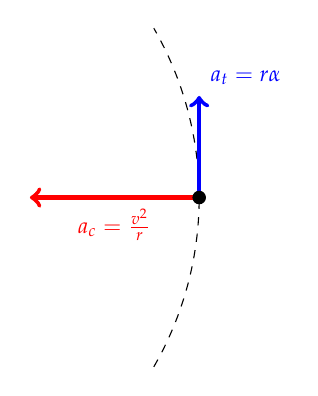
\begin{tikzpicture}[scale=4.3]
      \draw[dashed] (.866,-.5) arc(-30:30:1);
      \draw[ultra thick, red,->] (1,0)--(.5,0)
      node[midway,below]{\footnotesize $a_c=\frac{v^2}{r}$};
      \draw[ultra thick, blue,->] (1,0)--(1,.3)
      node[pos=1,above right]{\footnotesize $a_t=r\alpha$};
      \fill (1,0) circle(.02);
    \end{tikzpicture}
    
    \column{.75\textwidth}
    \textcolor{red}{\textbf{Centripetal acceleration} $a_c$}
    \begin{itemize}
    \item Depends on radius of curvature $r$ and instantaneous speed $v$.
    \item The direction of $a_c$ is toward the center of the circle.
    \end{itemize}
    \textcolor{blue}{\textbf{Tangential acceleration} $a_t$}
    \begin{itemize}
    \item Depends on radius $r$  and angular acceleration $\alpha$.
    \item The direction of the acceleration is tangent to the circle, which
      is the same as the velocity vector $\mb{v}$.
    \end{itemize}
  \end{columns}
\end{frame}



\begin{frame}{How to Solve Circular Motion Problems}
  \begin{enumerate}
  \item Is there any circular motion?
  \item If so, the condition for circular motion is:

    \eq{-.2in}{
      \mb{F}_\mathrm{provided}=\mb{F}_\mathrm{required}
    }
    \begin{itemize}
    \item\vspace{-.2in}The \emph{provided} force comes from FBD
    \item The \emph{required} force comes from the centripetal force equation 
    \end{itemize}
  \item If the net force also has a tangential component, then there is also
    a change in angular velocity
  \end{enumerate}
\end{frame}



\begin{frame}{Example: Horizontal Motion}
  \begin{columns}
    \column{.4\textwidth}
    \pic{1}{puck-on-table.png}
    
    \column{.6\textwidth}
    \textbf{Example 2:} In the figure on the left, a mass
    $m_1=\SI{3.}{\kilo\gram}$ is rolling around a frictionless table with
    radius $R=\SI{1.}{\metre}$. with a speed of \SI{2.}{\metre\per\second}.
    What is the mass of the weight $m_2$?
  \end{columns}
\end{frame}



\begin{frame}{Banked Curves on Highways and Racetracks}
  \begin{columns}
    \column{.35\textwidth}
    \centering
    \pic{.8}{banked-turn-acceleration.png}\\
    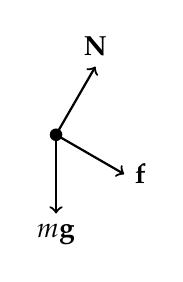
\begin{tikzpicture}
      \fill[black](0,0) circle(.08);
      \draw[thick,->,rotate=-30](0,0)--(0,1)node[pos=1,above]{$\mb{N}$};
      \draw[thick,->](0,0)--(0,-1)node[pos=1,below]{$m\mb{g}$};
      \draw[thick,->,rotate=60](0,0)--(0,-1)node[pos=1,right]{$\mb{f}$};
    \end{tikzpicture}
    \begin{tikzpicture}
      \draw[->](0,0)--(1,0) node[pos=1,right]{$x$};
      \draw[->](0,0)--(0,1) node[pos=1,above]{$y$};
    \end{tikzpicture}

    \column{.65\textwidth}
    No motion in the $y$ direction, therefore $\sum F_y=0$:

    \eq{-.25in}{
      N\cos\theta-f\sin\theta-w=0
    }

    Net force in the $x$ direction is the centripetal force,
    i.e.\ $\sum F_x=ma_c$

    \eq{-.25in}{
      N\sin\theta +f\cos\theta = \frac{mv^2}{r}
    }

    Friction force $\mb{f}$ may be static or kinetic, depending on the
    situation.
  \end{columns}
\end{frame}



\begin{frame}{Banked Curves on Highways and Racetracks}
  \begin{columns}
    \column{.35\textwidth}
    \centering
    \pic{.8}{banked-turn-acceleration.png}\\
    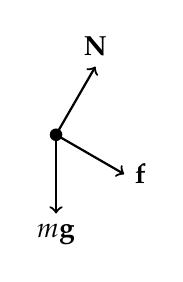
\begin{tikzpicture}
      \fill[black](0,0) circle(.08);
      \draw[thick,->,rotate=-30](0,0)--(0,1)node[pos=1,above]{$\mb{N}$};
      \draw[thick,->](0,0)--(0,-1)node[pos=1,below]{$m\mb{g}$};
      \draw[thick,->,rotate=60](0,0)--(0,-1)node[pos=1,right]{$\mb{f}$};
    \end{tikzpicture}
    \begin{tikzpicture}
      \draw[->](0,0)--(1,0) node[pos=1,right]{$x$};
      \draw[->](0,0)--(0,1) node[pos=1,above]{$y$};
    \end{tikzpicture}

    \column{.65\textwidth}
    For analysis, use the simplified equation for friction $f=\mu N$ (i.e.\
    assume either kinetic friction or maximum static friction), and weight
    $m\nb{g}$, the equations on the previous slides can be arranged as:

    \vspace{-.4in}{\Large
      \begin{align*}
        N\left(\cos\theta-\mu\sin\theta\right) &=mg\\
        N\left(\sin\theta+\mu\cos\theta\right) &=\frac{mv^2}{r}
      \end{align*}
    }
  \end{columns}
\end{frame}



\begin{frame}{Banked Curves on Highways and Racetracks}
  \begin{columns}
    \column{.35\textwidth}
    \centering
    \pic{.8}{banked-turn-acceleration.png}\\
    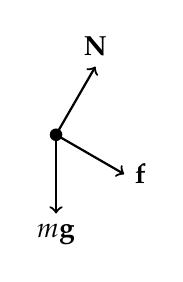
\begin{tikzpicture}
      \fill[black](0,0) circle(.08);
      \draw[thick,->,rotate=-30](0,0)--(0,1)node[pos=1,above]{$\mb{N}$};
      \draw[thick,->](0,0)--(0,-1)node[pos=1,below]{$m\mb{g}$};
      \draw[thick,->,rotate=60](0,0)--(0,-1)node[pos=1,right]{$\mb{f}$};
    \end{tikzpicture}
    \begin{tikzpicture}
      \draw[->](0,0)--(1,0) node[pos=1,right]{$x$};
      \draw[->](0,0)--(0,1) node[pos=1,above]{$y$};
    \end{tikzpicture}

    \column{.65\textwidth}
    Dividing the two equations removes both the normal force and mass terms:

    \eq{-.15in}{
      \frac{\sin\theta+\mu\cos\theta}{\cos\theta-\mu\sin\theta}
      =\frac{v^2}{rg}
    }

    The \emph{maximum} velocity $v_{\text{max}}$ can be expressed as:

    \eq{-.2in}{
      \boxed{v_\text{max}=
        \sqrt{rg\frac{\sin\theta+\mu\cos\theta}{\cos\theta-\mu\sin\theta}}
      }
    }

    Note that $v_\text{max}$ does not depend on mass.
  \end{columns}
\end{frame}



\begin{frame}{Banked Curves on Highways and Racetracks}
  In the limit of $\mu=0$ (frictionless case), the equation reduces to:

  \eq{-.1in}{
    \boxed{ v_\text{max}=\sqrt{rg\tan\theta} }
  }

  And in the limit of a flat roadway with no banking ($\theta=0$,
  $\sin\theta=0$ and $\cos\theta=1$), the equation reduces to:

  \eq{-.2in}{
    \boxed{ v_\text{max}=\sqrt{\mu rg} }
  }
\end{frame}



\section{Vertical Circles}

\begin{frame}{Vertical Circles}
  Circular motion with a horizontal path is straightforward. However, for
  vertical motion:
  \begin{itemize}
  \item Generally difficult to solve by dynamics and kinematics
  \item Instead, use conservation of energy to solve for speed $v$
  \item Then use the equation for centripetal force to find other forces
  \end{itemize}
  %If it is impossible to get the required centripetal force, then it could not
  %continue the circular motion
\end{frame}



\begin{frame}{What About a Pendulum?}
  A simple pendulum is also like a vertical circular motion problem.

  \vspace{.1in}\begin{columns}
    \column{.35\textwidth}
    \begin{tikzpicture}[scale=.8]
      \fill[pattern=north east lines] (-1,0) rectangle (1,0.2);
      \draw[very thick](-1,0)--(1,0);
      \begin{scope}[rotate=20]
        \draw[thick](0,0)--(0,-5);
        \tikzstyle{balloon}=[ball color=red!70!black];
        \shade[balloon] (0,-5) circle (.2);% node[below right]{$m$};
        \draw[->,very thick,red!70!black](0,-5)--(0,-3.3)
        node[pos=1,left]{\footnotesize $\mb{T}$};
        \draw[->,very thick,red!70!black,rotate around={-20:(0,-5)}]
        (0,-5)--(0,-6.5)
        node[pos=1,below]{\footnotesize $m\mb{g}$};
      \end{scope}
      \draw[dashed,thin](0,0)--(0,-5);
      \draw[dashed,thin](3.54,-3.54) arc(315:225:5);
      \draw[->](0,-2) arc(270:290:2) node[midway,below]{$\theta$};
    \end{tikzpicture}

    \column{.65\textwidth}
    \begin{itemize}
    \item There are two forces act on the pendulum: weight $m\mb{g}$, and
    tension $\mb{T}$
    \item Speed of the pendulum at any height is found using conservation
      of energy
      \begin{itemize}
      \item $\mb{T}$ is $\perp$ to motion, therefore it does not do work
      \item Work is done by gravity (conservative!) alone
      \end{itemize}
    \item Tangential and centripetal accelerations are based on the net force
      along the angular and radial directions
    \end{itemize}
  \end{columns}
\end{frame}



\begin{frame}{Simple Pendulum}
  At the top of the swing, velocity $v$ is zero, therefore:
  
  \vspace{.1in}\begin{columns}
    \column{.5\textwidth}
    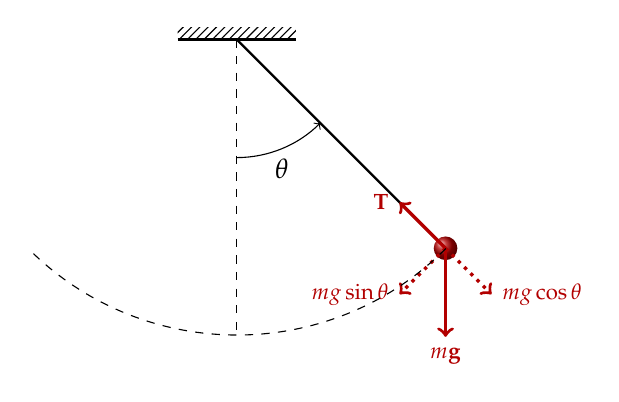
\begin{tikzpicture}[scale=.75]
      \fill[pattern=north east lines] (-1,0) rectangle (1,0.2);
      \draw[very thick](-1,0)--(1,0);
      \begin{scope}[rotate=45]
        \draw[thick](0,0)--(0,-5);
        \tikzstyle{balloon}=[ball color=red!70!black];    
        \shade[balloon] (0,-5) circle (.2);% node[below right]{$m$};
        \draw[dotted,->,very thick,red!70!black](0,-5)--(-1.1,-5)
        node[pos=1,left]{\footnotesize $mg\sin\theta$};
        \draw[dotted,->,very thick,red!70!black](0,-5)--(0,-6.1)
        node[pos=1,right]{\footnotesize $mg\cos\theta$};
        \draw[->,very thick,red!70!black](0,-5)--(0,-3.9)
        node[pos=1,left]{\footnotesize $\mb{T}$};
        \draw[->,very thick,red!70!black,rotate around={-45:(0,-5)}]
        (0,-5)--(0,-6.5)
        node[pos=1,below]{\footnotesize $m\mb{g}$};
      \end{scope}
      \draw[dashed,thin](0,0)--(0,-5);
      \draw[dashed,thin](3.54,-3.54) arc(315:225:5);
      \draw[->](0,-2) arc(270:315:2) node[pos=.5,below]{$\theta$};
    \end{tikzpicture}

    \column{.5\textwidth}
    Centripetal acceleration is also zero:

    \eq{-.2in}{
      a_c=\frac{v^2}{r}=0
    }

    and therefore the net force along the radial direction is zero. The tension
    force $T$ can be calculated:

    \eq{-.2in}{
      T=mg\cos\theta
    }
  \end{columns}
  At the highest point when $\theta$ is largest, tension is the lowest.
\end{frame}



\begin{frame}{Simple Pendulum}
  \begin{columns}
    \column{.5\textwidth}
    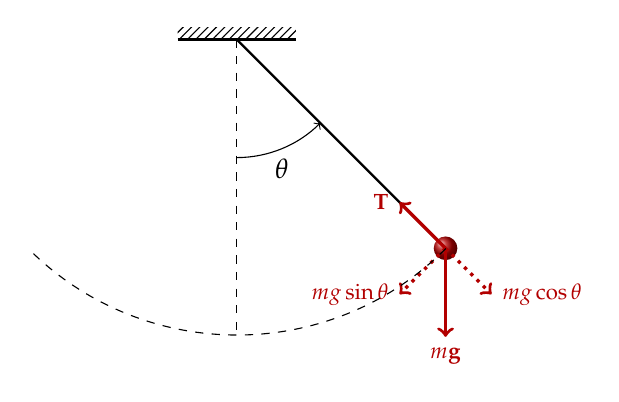
\begin{tikzpicture}[scale=.75]
      \fill[pattern=north east lines] (-1,0) rectangle (1,0.2);
      \draw[very thick](-1,0)--(1,0);
      \begin{scope}[rotate=45]
        \draw[thick](0,0)--(0,-5);
        \tikzstyle{balloon}=[ball color=red!70!black];    
        \shade[balloon] (0,-5) circle (.2); % node[below right]{$m$};
        \draw[dotted,->,very thick,red!70!black](0,-5)--(-1.1,-5)
        node[pos=1,left]{\footnotesize $mg\sin\theta$};
        \draw[dotted,->,very thick,red!70!black](0,-5)--(0,-6.1)
        node[pos=1,right]{\footnotesize $mg\cos\theta$};
        \draw[->,very thick,red!70!black](0,-5)--(0,-3.9)
        node[pos=1,left]{\footnotesize $\mb{T}$};
        \draw[->,very thick,red!70!black,rotate around={-45:(0,-5)}]
        (0,-5)--(0,-6.5)
        node[pos=1,below]{\footnotesize $m\mb{g}$};
      \end{scope}
      \draw[dashed,thin](0,0)--(0,-5);
      \draw[dashed,thin](3.54,-3.54) arc(315:225:5);
      \draw[->](0,-2) arc(270:315:2) node[pos=.5,below]{$\theta$};
    \end{tikzpicture}

    \column{.5\textwidth}
    In the tangential direction , there is a net force of $mg\sin\theta$,
    therefore, a tangential acceleration along that direction, with a
    magnitude of:

    \eq{-.25in}{
      a_t=g\sin\theta
    }

    \vspace{-.1in}This is the same acceleration as an object sliding down a
    frictionless ramp at an angle of $\theta$.
  \end{columns}
\end{frame}



\begin{frame}{Simple Pendulum}
  At the bottom of the swing, the velocity is at its maximum value,
  
  \vspace{.1in}\begin{columns}
    \column{.35\textwidth}
    \begin{tikzpicture}[scale=.8]
      \fill[pattern=north east lines] (-1,0) rectangle (1,0.2);
      \draw[very thick](-1,0)--(1,0);

      \draw[thick](0,0)--(0,-5);
      \tikzstyle{balloon}=[ball color=red!70!black];    
      \shade[balloon] (0,-5) circle (.2); %node[below right]{$m$};
      \draw[->,very thick,red!70!black](0,-5)--(0,-2.5)
      node[pos=1,right]{\footnotesize $\mb{T}$};
      \draw[->,very thick,red!70!black](0,-5)--(0,-6.5)
      node[pos=1,below]{\footnotesize $m\mb{g}$};

      \draw[dashed,thin](0,0)--(0,-5);
      \draw[dashed,thin](3.54,-3.54) arc(315:225:5);
    \end{tikzpicture}

    \column{.65\textwidth}
    \begin{itemize}
    \item Maximum centripetal acceleration:

      \eq{-.25in}{
        a_c=\frac{v^2}{r}
      }
    \item No tangential acceleration:

      \eq{-.25in}{
        a_t=0
      }
    \item At the lowest point, tension is the highest:

      \eq{-.3in}{
        T=w+F_c=m\left(g+\frac{v^2}{r}\right)
      }
    \end{itemize}
  \end{columns}
\end{frame}



\begin{frame}{Example Problem}
  \textbf{Example 4:} You are playing with a yo-yo with a mass $M$. The length
  of the string is $R$. You decide to see how slowly you can swing it in a
  vertical circle while keeping the string fully extended, even when it is at
  the top of its swing.
  \begin{enumerate}[a.]
  \item Calculate the minimum speed at which you can swing the yo-yo while
    keeping it on a circular path.
  \item Find the tension in the string when the yo-yo is at the side and at the
    bottom of its swing. 
  \end{enumerate}
\end{frame}



%\begin{frame}{Example Problem}
%  \textbf{Example 5:} A cord is tied to a pail of water, and the pail is swung
%  in a vertical circle of \SI{1.}{\metre}. What must be the minimum velocity of
%  the pail be at its highest point so that no water spills out?
%
%  \begin{enumerate}[(a)]
%  \item\SI{3.1}{\metre\per\second}
%  \item\SI{5.6}{\metre\per\second}
%  \item\SI{20.7}{\metre\per\second}
%  \item\SI{100.5}{\metre\per\second}
%  \end{enumerate}
%\end{frame}



\begin{frame}{Example: Roller Coaster}
  \textbf{Example 5:} A roller coaster car is on a track that forms a circular
  loop, of radius $R$, in the vertical plane. If the car is to maintain contact
  with the track at the top of the loop (generally considered to be a good
  thing), what is the minimum speed that the car must have at the bottom of the
  loop. Ignore air resistance and rolling friction.
  \begin{enumerate}[A.]
  \item $\sqrt{2gR}$
  \item $\sqrt{3gR}$
  \item $\sqrt{4gR}$
  \item $\sqrt{5gR}$
  \end{enumerate}
\end{frame}



%\begin{frame}{Example}
%  \textbf{Example 6:} A stone of mass $m$ is attached to a light strong string
%  and whirled in a \emph{vertical} circle of radius $r$. At the exact bottom of
%  the path, the tension of the string is three times the weight of the stone.
%  The stone's speed at that point is given by:
%  \begin{enumerate}[(a)]
%  \item $2\sqrt{gR}$
%  \item $\sqrt{2gR}$
%  \item $\sqrt{3gR}$
%  \item $4gR$
%  \end{enumerate}
%\end{frame}
\end{document}
